\documentclass[11pt,a4paper]{article}
\usepackage[margin=24mm]{geometry}
\usepackage{amsmath,amssymb,booktabs,tabularx,tikz,fontspec,xcolor}
\usetikzlibrary{positioning,arrows.meta}
\setmainfont{Noto Serif}
\usepackage[colorlinks=true,linkcolor=blue!50!black,urlcolor=blue!50!black,citecolor=blue!50!black,pdflang={en},pdfauthor={Aleksandr Strand},pdftitle={The Interface as a Resource for Discovery}]{hyperref}
\newcommand{\F}{\mathbb F}
\newcommand{\NP}{\mathrm{NP}}
\newcommand{\UP}{\mathrm{UP}}
\newcommand{\MP}[1]{\mathrm{Mod}_{#1}\mathrm P}
\newcommand{\LA}{\mathcal L_A}
\newcommand{\GI}{\mathrm{GI}_1}
\newcommand{\Sig}{\Sigma_2^{\mathrm P,A}}
\newcommand{\OR}{\mathrm{OR}}
\setlength\emergencystretch{2em}
\title{\textbf{The Interface as a Resource for Discovery}\\[5pt]\large Why eliminating ambiguity does not make hard problems easy}
\author{Aleksandr Strand\\
\small Independent researcher; a plain-language companion to\\
\small\textit{Recursive Switching and Modular Oracle Separations under $\NP=\UP$}}
\date{26 November 2026}
\begin{document}
\maketitle
\begin{abstract}
Imagine two computing systems looking at the same data table. Neither is given any new hidden facts. In this world, ambiguity has been removed: positive instances of problems in \(\NP\) can be represented with exactly one accepting witness each. The first system counts answers modulo a fixed prime \(p\), such as 2 or 3. It can even work with exponentially larger fields of the same characteristic, for example \(\F_3\to\F_{3^{100}}\). The second system can change the characteristic itself (\(\F_3,\F_5,\F_7,\ldots\)).

This companion explains the result of \textit{Recursive Switching and Modular Oracle Separations under NP = UP} without the full technical apparatus. Why can the first system not solve the seemingly simple empty-row problem in deterministic polynomial time, while the second can? The answer draws a precise distinction between scaling an interface and changing it. We separate the analytic proof, the components checked in Lean 4.36.0, and what remains open or conjectural for AI architecture.
\end{abstract}

\section{A library without ambiguity}
Imagine a vast library with \(N\) cabinets, each with exactly \(L\) numbered slots. In the model \(N=L=2^m\), so for \(m=100\) the scale is about \(10^{30}\). Each cabinet contains either one document serving as a witness or none at all. No duplicates, no conflicting copies.

Ask the librarian two questions that sound similar:
\begin{enumerate}
\item Is there a document in this particular cabinet \(u\)?
\item Is there at least one completely empty cabinet anywhere in the library?
\end{enumerate}
A yes to the first question has a short, unambiguous proof: open the right slot and show the document. In complexity theory, problems with efficiently checkable witnesses form the class \(\NP\). Its unambiguous counterpart, where every yes-instance has exactly one accepting computation, is \(\UP\).

The second question is different. To establish that cabinet \(u\) is empty, showing one document will not help: every slot must be ruled out.
\[
 \underbrace{\exists u}_{\text{there is a cabinet}}\qquad
 \underbrace{\forall v}_{\text{in every one of its slots}}\qquad A(u,v)=0.
\]
This alternation between existence and universality puts the task on the second level of the polynomial hierarchy, \(\Sigma_2^{\mathrm P}\).

\begin{figure}[htbp]\centering
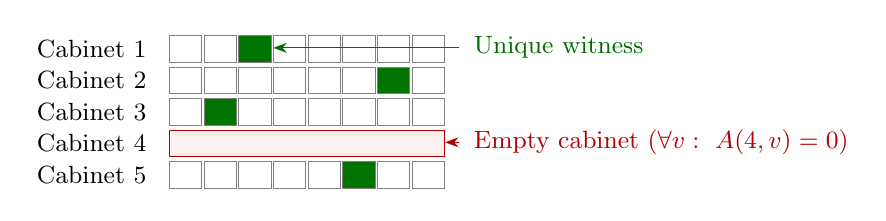
\begin{tikzpicture}[font=\small]
\foreach \r/\c in {1/3,2/7,3/2,4/0,5/6}{
\node[anchor=east] at (0,-.4*\r+.2) {Cabinet \r};
\foreach \j in {1,...,8}{
\ifnum\j=\c\relax
\fill[green!45!black] ({.44*(\j-1)+.17},{-.4*\r+.025}) rectangle +(0.41,.34);
\fi
\draw[gray] ({.44*(\j-1)+.17},{-.4*\r+.025}) rectangle +(0.41,.34);
}}
\draw[red!70!black,fill=red!6] (.17,-1.575) rectangle (3.66,-1.235);
\draw[green!42!black,-{Stealth}] (3.85,-.19) -- (1.49,-.19);
\node[anchor=west,text=green!42!black] at (3.91,-.19) {Unique witness};
\draw[red!70!black,-{Stealth}] (3.85,-1.39) -- (3.67,-1.39);
\node[anchor=west,text=red!70!black] at (3.91,-1.39) {Empty cabinet (\(\forall v:\ A(4,v)=0\))};
\end{tikzpicture}
\caption{Every nonempty cabinet holds exactly one document (green). The \(\Sigma_2^{\mathrm P}\) task is to distinguish a library with no empty cabinets from one with at least one.}
\end{figure}

If every \(\NP\) question can be represented unambiguously (\(\NP=\UP\)) and the observer can count accepting branches at once modulo any one fixed prime \(p\), surely finding an empty cabinet should be easy? The main result shows that it need not be.

\section{What exactly does the main theorem say?}
In a relativized setting, every machine can consult a common mathematical oracle \(A\), as in the classic work of Baker, Gill, and Solovay~\cite{bgs}. We construct an oracle \(A\) with the acyclic unique-witness invariant \(\GI\), based on the construction of Glaßer and Wechsung~\cite{gw}, for which two statements hold simultaneously:
\[
 \NP^A=\UP^A\quad\text{and}\quad
 \LA\in\Sig\setminus\bigcup_{p\text{ prime}}\MP p^A .
\]
Why \(\Sig\), rather than \(\NP^A\)? When \(\NP^A=\UP^A\), every language in \(\NP^A\) has a machine with zero or one accepting branch, and 0 and 1 differ modulo any \(p\ge 2\). Thus \(\NP^A\), and even the whole second-level deterministic class \(\Delta_2^{\mathrm P,A}=\mathrm P^{\NP^A}\), lies in \(\MP p^A\) for each prime \(p\). The second level is therefore the first at which this kind of resistance to modular counting is possible under \(\NP^A=\UP^A\).

\begin{table}[htbp]\small\centering
\begin{tabularx}{\linewidth}{@{}>{\raggedright\arraybackslash}p{.47\linewidth} >{\raggedright\arraybackslash}X@{}}
\toprule Observer's resource in world \(A\) & Can it decide the empty-cabinet problem \(\LA\)?\\
\midrule Unique witnesses for all of \(\NP^A\) (\(\NP^A=\UP^A\)) & The identity holds by construction.\\
Counting modulo 2, 3, or any one fixed prime \(p\) & Insufficient for any polynomial-time machine of that modular class.\\
Algebraic access over \(\F_p\to\F_{p^k}\) (fixed \(p\)) & Insufficient in the deterministic setting.\\
Adding randomness (\(\mathrm{RP}^{\widetilde A_{\F_3}}\)) & Solvable (Valiant--Vazirani isolation).\\
Changing the field characteristic (\(\F_3,\F_5,\F_7,\ldots\)) & Solvable deterministically (Chinese remainder theorem).\\
\bottomrule
\end{tabularx}
\caption{What does and does not break the barrier in the constructed world \(A\).}
\end{table}

Nor is this just one exceptional oracle. By the Baire category theorem, the separating oracles form a dense \(G_\delta\) in the compact space \(X_{\GI}\) of compatible oracles. Whatever admissible finite fragment of the library you fix in advance, it can be completed into a world where the separation holds.



\section{How it is proved: four mechanisms}
The hard part is that \(A\) does not merely store the base cabinet matrix. To ensure \(\NP^A=\UP^A\), the construction uses an infinite recursive tower: each upper layer encodes answers to \(\NP\) questions about earlier layers with unique markers. If those markers are placed carelessly, for instance always in the first slot, even the second layer can trivially decide whether a particular cabinet is empty, defeating the separation. The proof keeps the tower under control in four steps.

\begin{figure}[htbp]\centering
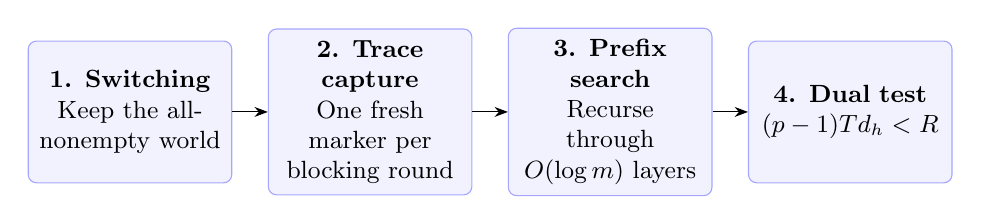
\begin{tikzpicture}[font=\small, node distance=4.5mm, stepbox/.style={draw=blue!35,fill=blue!5,rounded corners=3pt,text width=.19\linewidth,align=center,inner sep=4pt,minimum height=18mm}]
\node[stepbox] (a) {\textbf{1. Switching}\\Keep the all-nonempty world};
\node[stepbox,right=of a] (b) {\textbf{2. Trace capture}\\One fresh marker per blocking round};
\node[stepbox,right=of b] (c) {\textbf{3. Prefix search}\\Recurse through \(O(\log m)\) layers};
\node[stepbox,right=of c] (d) {\textbf{4. Dual test}\\\((p-1)Td_h<R\)};
\draw[-{Stealth}] (a)--(b); \draw[-{Stealth}] (b)--(c); \draw[-{Stealth}] (c)--(d);
\end{tikzpicture}
\caption{Four links in the argument from the base matrix to the modular lower bound.}
\end{figure}

\paragraph{1. Controlled deformation (Singleton-Preserving Switching).}
H\aa stad's classic method~\cite{hastad}, and its large-alphabet variants developed by Hirahara and Nanashima~\cite{hirahara}, simplify complicated formulas using random restrictions. In the Boolean case, such restrictions fix variables to 0 or 1. But we cannot fix cabinets to be empty: that would destroy the all-nonempty world. We instead use a one-sided projection, fixing some cabinets to be nonempty and leaving the others free. Empty states enter the auxiliary encoding measure used to prove injectivity, but are never fixed in the final projection.

\paragraph{2. Persistent Marker Knowledge and Trace Capture.}
At upper layers, positive conditions in a formula can guide negative queries straight to hidden markers. The algorithm remembers every true marker it has already exposed. Each new blocking round must therefore uncover a genuinely fresh marker, in a row not among those already disclosed as positive. A random split of the rows captures the whole trace with probability at least \([e(w+1)]^{-s}\).

\paragraph{3. Prefix recursion without a blowup.}
The strict acyclicity of \(\GI\) means that a computation running in \(T=\operatorname{poly}(m)\) time can reach at most \(h=O(\log m)\) nested layers. Instead of expanding formulas from upper layers into enormous base formulas, we binary-search for the first admissible term using prefix predicates from the previous layer. All oracle bits up to length \(T\) are thereby reduced simultaneously to decision trees of quasipolynomial depth \(d_h\le 2^{O(\log^4 m)}\) over a residual free cube of dimension \(R\ge 2^{m-O(\log^5 m)}\).

\paragraph{4. An algebraic ceiling on degree.}
By Fermat's little theorem the acceptance indicator of any \(\MP p^A\) machine can be represented by the integer polynomial \(C_M(A)^{p-1}\bmod p\), of degree at most \((p-1)Td_h\) in the remaining \(R\) free variables. Yet \(\OR_R(b)=1-\prod_{i=1}^R(1-b_i)\) requires full degree \(R\). The alternating functional
\[
 \Lambda_R(f)=\sum_{b\in\{0,1\}^R}(-1)^{|b|}f(b)
\]
annihilates every polynomial of degree below \(R\), but gives \(\Lambda_R(\OR_R)=-1\not\equiv0\pmod p\) for every \(p\ge 2\). For fixed \(p\) and sufficiently large \(m\), the degree bound \((p-1)Td_h\le 2^{O(\log^4 m)}\) is far below the dimension bound \(R\ge 2^{m-O(\log^5 m)}\). There must be an admissible world in the residual cube where the machine is wrong.

\section{Five shifts in what we can infer}
The result separates five ideas that everyday and engineering intuition often conflates.

\paragraph{1. Unambiguous knowledge is not easy global inference.}
Eliminating ambiguity (\(\NP^A=\UP^A\)) gives each positive local fact in the model one certificate. It does not make it easier to infer globally that certificates are absent.

\paragraph{2. The same information need not give the same computing power.}
In the algebrization model of Aaronson and Wigderson~\cite{aw}, and in the more recent multilinear barriers of Chen, Hu, and Ren~\cite{chr}, the multilinear extension \(\widetilde A\) is fully determined by the table \(A\) and adds no independent bits. Nevertheless, the way a machine can access the table is itself a computational resource.

\begin{figure}[htbp]\centering
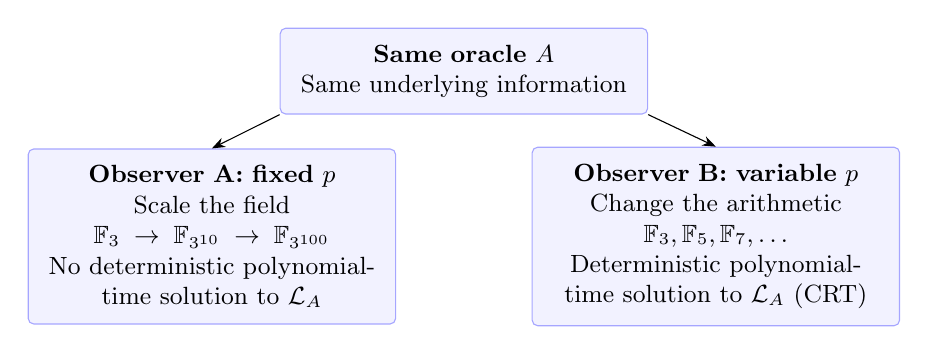
\begin{tikzpicture}[font=\small, box/.style={draw=blue!35,rounded corners=2pt,fill=blue!5,align=center,text width=.35\linewidth,inner sep=6pt}]
\node[box] (top) {\textbf{Same oracle \(A\)}\\Same underlying information};
\node[box] (a) at (-3.2,-2.1) {\textbf{Observer A: fixed \(p\)}\\Scale the field\\\(\F_3\to\F_{3^{10}}\to\F_{3^{100}}\)\\ No deterministic polynomial-time solution to \(\LA\)};
\node[box] (b) at (3.2,-2.1) {\textbf{Observer B: variable \(p\)}\\Change the arithmetic\\\(\F_3,\F_5,\F_7,\ldots\)\\ Deterministic polynomial-time solution to \(\LA\) (CRT)};
\draw[-{Stealth}] (top.south west)--(a.north); \draw[-{Stealth}] (top.south east)--(b.north);
\end{tikzpicture}
\caption{Increasing field size at fixed characteristic versus changing the characteristic of the interface.}
\end{figure}

\paragraph{3. Scaling within a language is not changing it.}
Increasing the field size from \(\F_p\) to \(\F_{p^k}\) does not make \(\LA\) accessible in deterministic polynomial time: \(\mathrm P^{\widetilde A^{[p]}}\subseteq\MP p^A\). The two ways of getting past this barrier considered here each change the model in kind: add randomness or permit changes in field characteristic.

\paragraph{4. Local simplicity is not global certifiability.}
After projection, each observable bit has degree at most \(d_h\). Even combining those bits as the polynomial-time machines in the proof do cannot reach degree \(R\), the degree of the global property \(\OR_R\).

\paragraph{5. An isolated anomaly is not topological typicality.}
The dense \(G_\delta\) in \(X_{\GI}\) shows that the separation is not a fragile, isolated counterexample: it is topologically typical among compatible worlds. Topological typicality should not be confused with probability one.



\section{What this means (and does not mean) for AI architecture}
An oracle complexity result does not itself prove any theorem about neural networks or LLMs. But it gives a precise mathematical model for a distinction that matters when designing agents.

\paragraph{An illustration with six empty cabinets.}
Imagine eight cabinets, six of them empty. An observer whose interface reports the empty-cabinet count modulo 2 sees \(6\bmod 2=0\); an observer counting modulo 3 sees \(6\bmod 3=0\). Even ten parallel agents cannot resolve this ambiguity by spending more tokens if all of them see only the same modulo-2 count. Change the interface to modulo 5 and it immediately reports \(6\bmod 5=1\ne 0\), distinguishing six empty cabinets from none in this example.

For AI agents, this distinguishes two kinds of scaling:
\begin{itemize}
\item \textbf{Quantitative scaling:} more tokens, attempts, memory, and copies of the agent within a fixed set of operations.
\item \textbf{Structural scaling:} detecting the limits of the current representation and making a verifiable switch to a different computational interface while retaining the original criterion for a correct answer.
\end{itemize}

For an agent that builds on earlier research, this suggests four layers of memory: factual (what we learned); procedural (how we did it); epistemic (why a particular class of methods hits a barrier); and structural (which change in representation removed the barrier).

\paragraph{A caveat for AI.}
In the mathematical model, the ability to change characteristic is built into the oracle interface. A real AI system has to build and verify the new interface, and those costs belong in the overall budget. Applying the principle to agent architecture is a research hypothesis in need of a controlled experiment, not a demonstrated advantage.

\section{Where the result stops}
A plain-language account should keep what has been proved separate from what has not.

\begin{table}[htbp]\small\centering
\begin{tabularx}{\linewidth}{@{}>{\raggedright\arraybackslash}p{.63\linewidth} >{\raggedright\arraybackslash}X@{}}
\toprule Claim & Actual status\\\midrule
Solution to the unrelativized P versus NP problem~\cite{cook} & No.\\
Proof that \(\mathrm{PH}^A\) is infinite under \(\NP^A=\UP^A\) (Grochow~\cite{grochow}) & No (open).\\
A general bypass of the algebrization barrier & No.\\
Proof that a new LLM architecture is superior & No (hypothesis).\\
End-to-end Lean formalization of the infinite oracle & Not yet.\\
Analytic proof of \(\Sig\not\subseteq\bigcup_p\MP p^A\) with \(\NP^A=\UP^A\) & Presented.\\
Machine checking of selected components and the finite bridge in Lean 4.36.0 & Seven modules; 45/45 audited theorems.\\
\bottomrule
\end{tabularx}
\caption{Established results, partial formalization, and open questions.}
\end{table}

Seven modules without imports in Lean 4.36.0 (45 audited theorems; zero errors; no \texttt{sorryAx}; no \texttt{Classical.choice}) machine-check selected combinatorial and algebraic components, as well as the conditional finite bridge (\texttt{UniformRecursiveBridge.lean}). The full probabilistic recursion and the construction of the infinite oracle are analytic. The work has not yet undergone external peer review.

\section{In place of a conclusion}
At the first level, we solve a hard problem by searching within a given language. At the next, we ask why the language itself cannot distinguish the states that matter. Only then can we ask the constructive question: what is the smallest change to the interface that makes previously inaccessible knowledge computable?

That distinction between the amount of data and the geometry of access to it is the central idea of this work.

earpage
\begin{thebibliography}{9}
\bibitem{aw} S. Aaronson and A. Wigderson. Algebrization: A new barrier in complexity theory. \textit{ACM Transactions on Computation Theory}, 1(1):2:1--2:54, 2009. \href{https://www.scottaaronson.com/papers/alg.pdf}{PDF}.
\bibitem{bgs} T. Baker, J. Gill, and R. Solovay. Relativizations of the P =? NP question. \textit{SIAM Journal on Computing}, 4(4):431--442, 1975. \href{https://epubs.siam.org/doi/10.1137/0204037}{DOI}.
\bibitem{chr} L. Chen, Y. Hu, and H. Ren. New algebrization barriers to circuit lower bounds via communication complexity of Missing-String. \textit{ITCS 2026}. \href{https://arxiv.org/abs/2511.14038}{arXiv:2511.14038}.
\bibitem{cook} S. Cook. The P versus NP problem. Clay Mathematics Institute, 2000. \href{https://www.claymath.org/wp-content/uploads/2022/06/pvsnp.pdf}{PDF}.
\bibitem{gw} C. Glaßer and G. Wechsung. Relativizing function classes. \textit{Journal of Universal Computer Science}, 9(1):34--50, 2003. \href{https://lib.jucs.org/issue/4069/}{JUCS 9(1)}.
\bibitem{grochow} J. A. Grochow. Polynomial-time axioms of choice and polynomial-time cardinality. \textit{Theory of Computing Systems}, 67, 2023. \href{https://arxiv.org/abs/2301.07123}{arXiv:2301.07123}.
\bibitem{hastad} J. H\aa stad. Almost optimal lower bounds for small depth circuits. In \textit{STOC 1986}, pp.~6--20, 1986.
\bibitem{hirahara} S. Hirahara and M. Nanashima. On worst-case learning in relativized Heuristica. In \textit{FOCS 2021}, pp.~751--758, 2021. \href{https://eccc.weizmann.ac.il/report/2021/161/download}{ECCC TR21-161}.
\end{thebibliography}
\end{document}
